\documentclass{standalone}
%%%%% tikz images %%%%%%
\usepackage{tikz, pgfplots} % for tikz images.
\usepackage{tikz-3dplot} % to draw a visual 3d image with tikz (not with pgfplots).
\usetikzlibrary{arrows,arrows.meta,decorations.pathmorphing,decorations.pathreplacing,decorations.shapes,decorations.markings,patterns,calc,fillbetween,intersections}
\usepgfplotslibrary{fillbetween, polar}
\pgfplotsset{compat=newest}

% \usepgfplotslibrary{external}
% \tikzexternalize
%%%%%%%%%%%%%%%%%%%%%%%%


\def\dist{34}
\def\size{1}
\def\a{2}
% golden ratio
\def\b{1.61803}
% plastic number
\def\c{1.32472}
\begin{document}
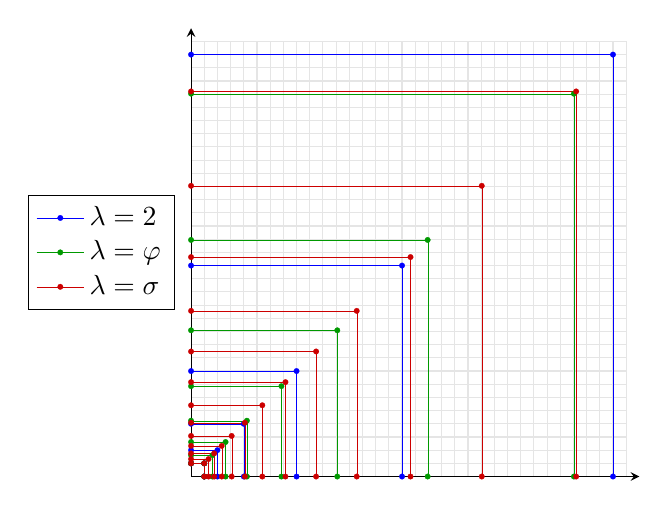
\begin{tikzpicture}
  \begin{axis}[
      axis lines=middle,
      xmin=0, xmax=\dist,
      ymin=0, ymax=\dist,
      xtick=\empty, ytick=\empty,
      ylabel={},
      xlabel={},
      % xlabel style={below right,font=\fontlabel},
      % ylabel style={left, xshift=-1em,font=\fontlabel},
      % xtick={0, 0.1, ..., 1},
      % ytick={0, 0.1, ..., 1},
      % % size of x and y ticks
      % xticklabel style={scale=\scaleticks},
      % yticklabel style={scale=\scaleticks},
      % include the 0 label
      % extra x ticks={0,1},
      % extra y ticks={0,1},
      axis on top,
      axis equal image,
      % legend (align text to the left)
      legend style={at={(-0.2, 0.5)}, anchor=center, legend columns=3, fill=none,transpose legend,/tikz/every even column/.append style={column sep=0.2cm}},
      % text to the left of the legend
      legend cell align={left},
      % legend font scale
    ]
    \draw[step=1.0,black!10,thin] (0,0) grid (\dist-1, \dist-1);
    \addplot[mark =*,mark size=\size, blue, ultra thin] coordinates {
        (0,1)
        (1,1)
        (1,0)
      };
    \addplot[mark =*,mark size=\size, green!60!black, ultra thin] coordinates {
        (0,1)
        (1,1)
        (1,0)
      };
    \addplot[mark =*,mark size=\size,  red!80!black, ultra thin] coordinates {
        (0,1)
        (1,1)
        (1,0)
      };
    \foreach \n in {0,1,...,5}{
        \addplot[mark =*,mark size=\size, blue, ultra thin] coordinates {
            (0,\a^\n)
            (\a^\n, \a^\n)
            (\a^\n,0)
          };
      }
    \foreach \n in {0,1,...,8}{
        \addplot[mark =*,mark size=\size, green!60!black, ultra thin] coordinates {
            (0,\b^\n)
            (\b^\n, \b^\n)
            (\b^\n,0)
          };
      }
    \foreach \n in {0,1,...,13}{
        \addplot[mark =*,mark size=\size, red!80!black, ultra thin] coordinates {
            (0,\c^\n)
            (\c^\n, \c^\n)
            (\c^\n,0)
          };
      }
    \legend{$\lambda=2$,$\lambda=\varphi$,$\lambda=\sigma$}
    % \addplot [only marks, mark=*, mark size=\size, draw=black, fill=blue, ultra thin] coordinates {
    %     (0,1)
    %     (0,2)
    %     (0,4)
    %     (0,8)
    %     (0,16)
    %     (0,32)
    %     (1,0)
    %     (2,0)
    %     (4,0)
    %     (8,0)
    %     (16,0)
    %     (32,0)
    %   };


  \end{axis}
\end{tikzpicture}
\end{document}
